\chapter{Results}
\label{ch:results}

All results in this chapter are computed on participants who were not used for training: the internal test set (2,286 participants, 332 converters) and the nine held-out centres (4,064 participants, 545 converters). Intervals are 95\% bootstrap intervals. Every number can be traced to a result file in the project repository.

\section{Comparison of models}

\begin{table}[H]
\centering\small
\caption{Discrimination and calibration of the five models.}
\label{tab:models_res}
\begin{tabular}{@{}lccccc@{}}
\toprule
 & \multicolumn{3}{c}{Test set} & \multicolumn{2}{c}{Held-out centres} \\
\cmidrule(lr){2-4}\cmidrule(l){5-6}
Model & AUROC (95\% CI) & AUPRC & Brier & AUROC & Brier \\
\midrule
Logistic regression & 0.936 (0.924--0.949) & 0.721 & 0.066 & 0.945 & 0.060 \\
Random forest & 0.932 (0.919--0.944) & 0.704 & 0.070 & 0.940 & 0.064 \\
XGBoost & 0.938 (0.925--0.948) & 0.713 & 0.066 & 0.946 & 0.059 \\
Multilayer perceptron & 0.938 (0.926--0.949) & 0.721 & 0.066 & 0.946 & 0.059 \\
FT-Transformer & 0.939 (0.927--0.949) & 0.720 & 0.066 & 0.945 & 0.061 \\
\bottomrule
\end{tabular}
\end{table}

The five models perform almost identically, and their confidence intervals overlap almost completely (Table~\ref{tab:models_res}). The deep-learning models did not outperform logistic regression or gradient boosting on these data. For reference, always predicting the training event rate gives a Brier score of 0.124, so all models are substantially better calibrated than a constant prediction.

\begin{figure}[H]
\centering
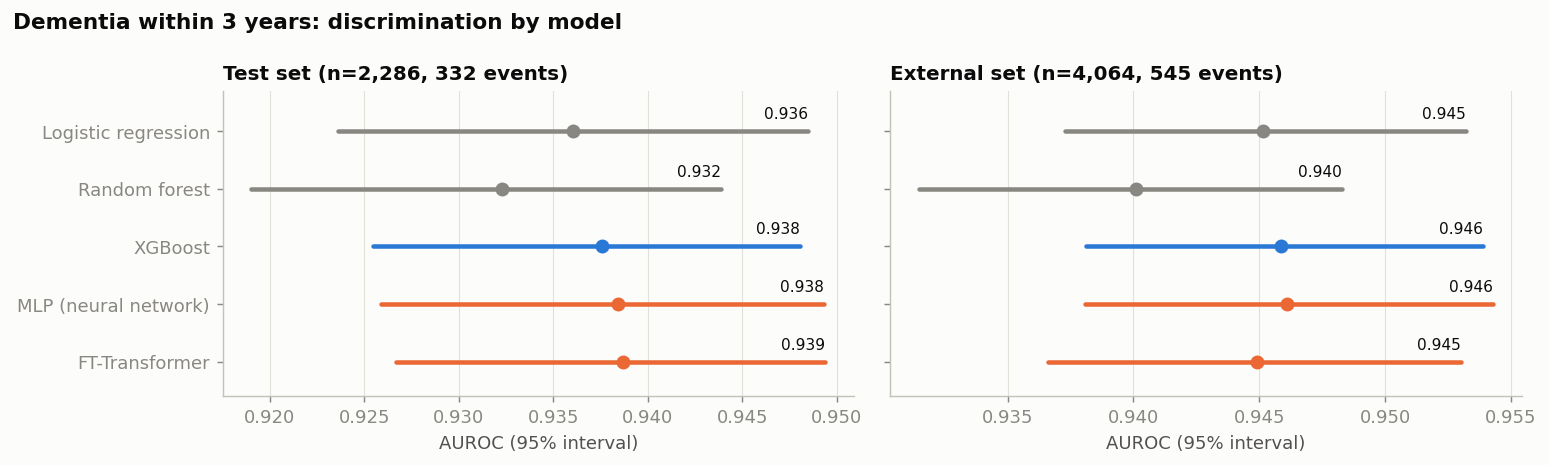
\includegraphics[width=\textwidth]{06_model_comparison.png}
\caption{AUROC and AUPRC of the five models on the test set and the held-out centres.}
\label{fig:models}
\end{figure}

\section{Performance by diagnosis at the index visit}
\label{sec:res_groups}

The cohort combines cognitively normal participants, who rarely convert (1.6\%), with participants with MCI, who often do (41.5\%). Diagnosis alone therefore separates converters from non-converters well: a model given only the diagnosis reaches an AUROC of 0.84. Table~\ref{tab:groups} reports XGBoost separately within each group.

\begin{table}[H]
\centering\small
\caption{XGBoost by diagnosis at the index visit (participants / converters).}
\label{tab:groups}
\begin{tabular}{@{}lcccc@{}}
\toprule
 & \multicolumn{2}{c}{Test set} & \multicolumn{2}{c}{Held-out centres} \\
\cmidrule(lr){2-3}\cmidrule(l){4-5}
Group & $n$ / events & AUROC (95\% CI) & $n$ / events & AUROC (95\% CI) \\
\midrule
All not demented & 2,286 / 332 & 0.937 (0.925--0.948) & 4,064 / 545 & 0.946 (0.938--0.954) \\
Cognitively normal & 1,411 / 24 & 0.884 (0.819--0.936) & 2,624 / 37 & 0.876 (0.823--0.918) \\
MCI & 732 / 289 & 0.835 (0.807--0.862) & 1,291 / 496 & 0.846 (0.824--0.867) \\
\bottomrule
\end{tabular}
\end{table}

Within MCI the AUROC is about 0.84, which is the more informative estimate of how well the model ranks risk among people who are already impaired. Within the cognitively normal group the AUROC is about 0.88, but it rests on only 24 and 37 events and the intervals are wide; with an event rate of 1.6\% the average precision is only 0.15 to 0.19, so most participants flagged as high risk would not convert. Models trained only on normal participants (AUROC 0.876 and 0.881) or only on MCI participants (0.829 and 0.838) gave the same picture, so the group results are not an artefact of mixing the groups during training.

\section{What drives the prediction}

\subsection{Feature categories}

\begin{table}[H]
\centering\small
\caption{Contribution of each feature category (XGBoost, test set unless stated).}
\label{tab:ablation}
\begin{tabular}{@{}lccc@{}}
\toprule
Category & Alone & Gain when added to all others (test) & Gain (held-out centres) \\
\midrule
Cognitive tests & 0.896 & $+0.022$ ($+0.015$ to $+0.029$) & $+0.019$ ($+0.013$ to $+0.024$) \\
Clinical stage (CDR-SB, diagnosis) & 0.897 & $+0.015$ ($+0.007$ to $+0.023$) & $+0.021$ ($+0.015$ to $+0.027$) \\
Demographics & 0.671 & $+0.010$ ($+0.006$ to $+0.015$) & $+0.009$ ($+0.006$ to $+0.013$) \\
Genetics (APOE) & 0.645 & $+0.003$ ($+0.002$ to $+0.004$) & $+0.001$ ($-0.000$ to $+0.002$) \\
Cardiovascular and medical & 0.626 & $+0.001$ ($-0.000$ to $+0.003$) & $+0.001$ ($+0.000$ to $+0.002$) \\
\bottomrule
\end{tabular}
\end{table}

Cognitive tests and clinical stage each reach an AUROC near 0.90 on their own and make the largest unique contributions (Table~\ref{tab:ablation}, Figure~\ref{fig:groups}). Because these two categories overlap, removing either one costs little; removing both together, so that the model has no information about current cognition, lowers the AUROC from 0.937 to 0.746 on the test set (0.744 on the held-out centres). Within the normal and MCI groups the corresponding values are 0.783 and 0.638. The model therefore relies mainly on how impaired a person already is at the index visit. Because all these variables are recorded at the index visit and the outcome occurs later, this is not leakage, but it means the model is best described as estimating short-term progression given the current clinical stage.

\begin{figure}[H]
\centering
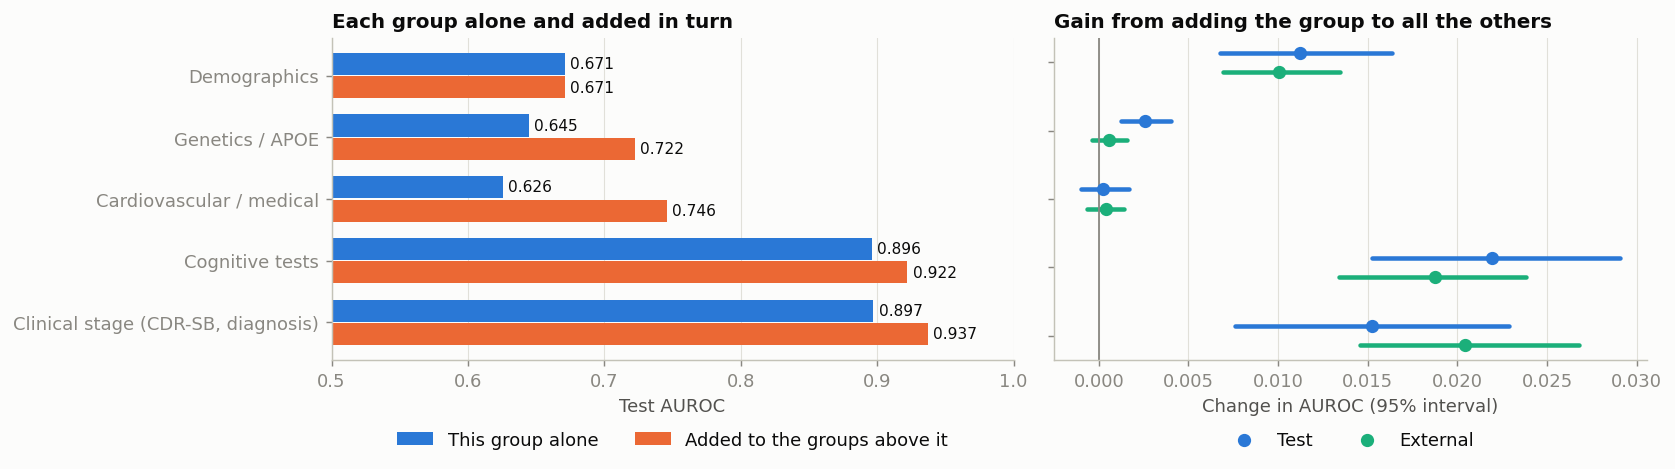
\includegraphics[width=\textwidth]{06_feature_groups.png}
\caption{Left: AUROC of each category alone and added cumulatively. Right: gain in AUROC from adding each category to all the others.}
\label{fig:groups}
\end{figure}

\subsection{Cardiovascular information (research question 1)}

On its own, the cardiovascular category carries some signal (AUROC 0.626). Added to demographics and APOE only, before any cognitive information, it improved the AUROC by 0.024 on the test set (0.011 to 0.039), but by only 0.004 at the held-out centres ($-0.006$ to $0.015$). Once cognitive information is present its contribution falls to about 0.001, with an interval that includes zero on the test set. Within the cognitively normal group the gain was 0.008 on the test set and 0.003 at the held-out centres, with intervals spanning zero. In this cohort and prediction setting, therefore, cardiovascular and medical history added little incremental predictive value beyond current cognitive status. This finding does not imply that vascular health is unimportant for the brain: the participants enter at a median age of 71, mid-life exposure is not observed, and vascular damage that has already occurred is likely to be reflected in the cognitive scores.

\subsection{Shapley explanations}

\begin{table}[H]
\centering\small
\caption{Share of mean absolute SHAP value by category (test set, 2,286 participants).}
\label{tab:shap}
\begin{tabular}{@{}lc@{}}
\toprule
Category & Share \\
\midrule
Clinical stage (CDR-SB, diagnosis) & 40.8\% \\
Cognitive tests & 35.0\% \\
Demographics & 15.5\% \\
Cardiovascular and medical & 5.1\% \\
Genetics & 3.5\% \\
\bottomrule
\end{tabular}
\end{table}

The most important individual features were CDR-SB, MCI status, the memory score, age and the executive score. The ranking was stable across eight bootstrap refits (Spearman correlation with the main model 0.89 to 0.97; 8 to 10 of the top ten features shared). Some associations are not causal: lower BMI was associated with higher predicted risk, which is consistent with weight loss in the years before a dementia diagnosis rather than a protective effect of higher weight.

\section{Cognitive Decline as the Outcome}

Table~\ref{tab:decline} reports the secondary outcome, a rise of at least one point in CDR-SB within three years. The cohort is slightly larger than for dementia (20,355 participants, 5,035 events) because the outcome can be observed in people who decline without reaching dementia.

\begin{table}[H]
\centering\small
\caption{XGBoost for CDR-SB worsening of at least one point within three years (participants / events).}
\label{tab:decline}
\begin{tabular}{@{}lcccc@{}}
\toprule
 & \multicolumn{2}{c}{Test set} & \multicolumn{2}{c}{Held-out centres} \\
\cmidrule(lr){2-3}\cmidrule(l){4-5}
Group & $n$ / events & AUROC (95\% CI) & $n$ / events & AUROC (95\% CI) \\
\midrule
All not demented & 2,375 / 572 & 0.858 (0.841--0.874) & 4,272 / 1,035 & 0.885 (0.875--0.896) \\
Cognitively normal & 1,459 / 129 & 0.760 (0.714--0.805) & 2,690 / 215 & 0.831 (0.806--0.856) \\
MCI & 766 / 399 & 0.748 (0.712--0.779) & 1,411 / 774 & 0.749 (0.723--0.776) \\
\bottomrule
\end{tabular}
\end{table}

Decline is harder to predict than dementia, as expected for an outcome that includes small changes in a rating scale. The cognitively normal group is much better represented here (129 and 215 events instead of 24 and 37), so the estimate of 0.76 to 0.83 in that group is more reliable than the corresponding dementia result. Logistic regression gave almost the same result (0.854 and 0.883). The pattern of contributions matched the dementia outcome: cognitive tests made the largest unique contribution ($+0.029$ on the test set), and the cardiovascular category added nothing measurable ($+0.0004$, interval $-0.003$ to $+0.003$; held-out centres $0.000$).

\subsection{Predicted Change in CDR-SB}

For the 1,863 test participants and 3,231 held-out participants with a visit near the three-year mark, the mean change in CDR-SB was 0.48 and 0.63 points, and three quarters showed no change or an improvement. The regression model reduced the mean absolute error from 0.69 (predicting no change) to 0.60 on the test set and from 0.83 to 0.72 at the held-out centres, with $R^2$ of 0.23 and 0.18 and a Spearman correlation of 0.45. Within MCI the error fell from 1.90 to 1.59 points. Within cognitively normal participants, whose scores rarely change, the model was no better than predicting no change (0.17 against 0.17). The progression estimate is therefore informative for people who are already impaired and adds little for people who are not.

\section{Modality-Encoder Fusion Network}

The fusion network reached an AUROC of 0.934 (0.920--0.946) on the test set and 0.943 (0.935--0.951) at the held-out centres for dementia, against 0.937 and 0.946 for XGBoost; within MCI 0.831 and 0.837, and within cognitively normal participants 0.846 and 0.874. Its progression head reduced the mean absolute error from 0.72 to 0.65 on the test set. With modalities removed it behaved like the modality-dropout XGBoost model: without any cognitive information its AUROC was 0.72 and its Brier score 0.114, close to the specialist value.

The attention weights, intended as an explanation of how much the network relied on each modality, were nearly equal: between 18\% and 21\% for every modality, on both evaluation sets and in every diagnostic group. They stayed almost equal even when the cognitive modalities were missing, because the learned missing tokens themselves carry the information. The attention weights therefore do not reveal which modality drives a prediction, in line with the wider observation that attention weights are not reliable explanations. The ablation results and SHAP values, which show that cognitive information dominates, remain the explanations used in this work. The fusion network demonstrates that the proposed architecture works and copes with missing modalities, but it offers no gain in accuracy over gradient-boosted trees on these data.

\section{Longitudinal information}

On landmark visits preceded by at least two earlier visits (test: 1,205 participants, 166 events; held-out centres: 2,254 participants, 326 events), adding the visit history produced only small changes (Table~\ref{tab:long}).

\begin{table}[H]
\centering\small
\caption{Effect of earlier visits (paired gain over the landmark-only model).}
\label{tab:long}
\begin{tabular}{@{}lcc@{}}
\toprule
Model & Test AUROC (gain) & Held-out AUROC (gain) \\
\midrule
XGBoost, landmark visit only & 0.919 & 0.953 \\
XGBoost with trajectory features & 0.922 ($+0.003$; $-0.006$ to $+0.011$) & 0.956 ($+0.003$; $-0.001$ to $+0.007$) \\
GRU over the visit sequence & 0.920 ($+0.000$; $-0.011$ to $+0.010$) & 0.958 ($+0.005$; $+0.001$ to $+0.008$) \\
\bottomrule
\end{tabular}
\end{table}

When current scores are known, the path that led to them adds little for a three-year prediction. This does not show that longitudinal modelling is of no value; a longer horizon, an earlier disease stage or more frequent measurement could give a different result.

\section{PET measures (research question 2)}
\label{sec:res_pet}

On its own, amyloid status is strongly associated with progression: among participants with MCI in the held-out sets, about 34\% of amyloid-positive participants received a dementia diagnosis within two years, compared with about 7\% of amyloid-negative participants (36\% and 9\% under the strict scan-matching rule). Added to the clinical model, however, the PET measures did not produce a clear improvement under either matching rule. For example, with strict matching and a three-year horizon, the AUROC at the held-out centres was 0.939 without and 0.946 with amyloid (191 participants, 27 events; paired gain $-0.007$ to $+0.024$). The final late-fusion model scored 0.964 against 0.944 for the clinical model on 243 held-out scanned participants with 33 events, a gain of 0.020 whose interval ($-0.009$ to $+0.066$) includes zero. A modest benefit cannot be excluded, but it could not be demonstrated with the follow-up currently available.

\section{Validation}

\subsection{Subgroups}

\begin{table}[H]
\centering\small
\caption{XGBoost AUROC by subgroup.}
\label{tab:subgroups}
\begin{tabular}{@{}lcc@{}}
\toprule
Subgroup & Test (n / events) & Held-out centres (n / events) \\
\midrule
Female & 0.950 (1,338 / 162) & 0.947 (2,507 / 272) \\
Male & 0.919 (948 / 170) & 0.941 (1,557 / 273) \\
Age under 65 & 0.976 (467 / 46) & 0.958 (1,067 / 56) \\
Age 65--74 & 0.952 (963 / 99) & 0.956 (1,463 / 191) \\
Age 75--84 & 0.904 (732 / 157) & 0.937 (1,044 / 191) \\
Age 85 and over & 0.852 (124 / 30) & 0.888 (490 / 107) \\
White & 0.933 (1,813 / 273) & 0.943 (3,347 / 499) \\
Black & 0.948 (304 / 31) & 0.951 (471 / 26) \\
Education 12 years or less & 0.926 (400 / 92) & 0.920 (744 / 137) \\
Education over 16 years & 0.951 (937 / 112) & 0.960 (1,551 / 188) \\
APOE $\varepsilon$4 carrier & 0.915 (762 / 150) & 0.933 (1,402 / 277) \\
\bottomrule
\end{tabular}
\end{table}

Discrimination was similar across sex, race and education. It was lower in the oldest participants and in APOE $\varepsilon$4 carriers, both groups with a higher baseline risk.

\subsection{Calibration and clinical usefulness}

On the test set the mean predicted risk (14.5\%) equalled the observed rate (14.5\%), with a calibration slope of 1.01 and intercept of 0.009. At the held-out centres the model over-predicted slightly (15.0\% predicted, 13.4\% observed; slope 1.10). Using a risk threshold of 20\%, the model flagged 22\% of test participants with a sensitivity of 83\%, specificity of 88\%, positive predictive value of 55\% and negative predictive value of 97\% (held-out centres: 90\%, 87\%, 52\% and 98\%). Decision curve analysis showed a higher net benefit than treating everyone or no one across all thresholds examined, from 2\% to 60\%, on both evaluation sets.

\section{Missing information}

\begin{table}[H]
\centering\small
\caption{Brier score when categories are missing (test set; lower is better).}
\label{tab:dropout}
\begin{tabular}{@{}lccc@{}}
\toprule
Available information & Standard model & Modality dropout & Specialist model \\
\midrule
Everything & 0.066 & 0.067 & 0.066 \\
No cognitive tests & 0.082 & 0.077 & 0.080 \\
No clinical stage & 0.185 & 0.076 & 0.074 \\
No cognitive information at all & 0.441 & 0.115 & 0.111 \\
Demographics only & 0.444 & 0.120 & 0.118 \\
\bottomrule
\end{tabular}
\end{table}

A standard model given missing inputs at prediction time produced badly calibrated risks when cognitive information was absent, worse than predicting the base rate (Brier 0.124). The model trained with modality dropout stayed close to a specialist model retrained for each situation (Table~\ref{tab:dropout}), with almost no loss when all information is present. This model is used in the clinician interface.

\section{Sensitivity analyses}
\label{sec:res_sens}

\textbf{Censored participants.} A Cox model fitted on all eligible participants, including those followed for less than three years, reached a concordance index of 0.891 on the test set and 0.903 at the held-out centres. Removing the cardiovascular category changed the concordance by 0.001 ($-0.001$ to $0.003$) and 0.000 ($-0.001$ to $0.002$). Hazard ratios per standard deviation were 1.37 for CDR-SB, 0.76 for the memory score, 1.40 for age and 1.20 for each APOE $\varepsilon$4 allele, while hypertension (0.995, 0.953--1.038), diabetes and stroke had hazard ratios close to one.

\textbf{Reversed diagnoses.} A clinical diagnosis can be revised. Of the 2,818 converters, 217 (7.7\%) were recorded as not demented at a later visit. Excluding them, XGBoost reached an AUROC of 0.947 on the test set and 0.950 at the held-out centres (MCI: 0.839 and 0.851). The conclusions do not depend on reversed diagnoses.

\textbf{Variables close to the diagnosis.} Adding the daily-function questionnaire, independence, memory complaints and Alzheimer's medication increased the AUROC by 0.006 on the test set and 0.005 at the held-out centres. These variables were therefore left out of the main model with little loss of accuracy.
